% !TEX root = Thesis.tex

%==============================================================================
\chapter{Diffraction of a \acl{bec} with a one-dimensional Optical lattice}
\label{chap:one_dimensional_lattices}
%==============================================================================
In ultracold atoms physics, Optical lattices are defined as periodic standing wave potentials generated by interfering laser beams. Its use allows to replicate results from solid state physics, with the interaction between an ultracold atomic ensemble and an optical lattice being equivalent to the role of electrons in an atomic lattice (i.e. a solid-state crystal) \cite{Lewenstein2007, Bloch2008,Morsch2006}.  However, the use of ultracold systems presents some advantages when comparing with those used in solid state physics. The main one being the capability of changing the optical lattice properties, by simply adjusting parameters like the intensity and detuning of the laser beams forming it. An additional advantage of ultracold atomic systems is the non-existence of crystal defects, which can be a big source of noise in solid states systems \cite{VanDerZiel1978}. This experiment will seek to study how an erbium \ac{bec} behaves when interacting with a one-dimensional optical lattice. In this chapter, an introduction describing the theory behind optical lattices will be shown. After this, it follows a brief description of the implemented set up to form the lattice by using the \SI{841}{\nano\meter} erbium transition (see Table \ref{tab:Transitions}).


\section{Theoretical description of an Optical lattice}

As it can be seen in Figure \ref{fig:lattice_beams}, generating an optical lattice requires the use of two interfering laser beams, with a detuning $\delta$ from the used atomic transition (in this case the \SI{841}{\nano\meter} erbium transition). The main parameter that allows to characterize the experiment is known as the lattice depth $U_0$ and will be determined theoretically in this section by assuming some approximations in the atom behaviour. Moreover, the lattice prosperities can be changed by adjusting the optical intensity of the beams as well as the frequency detuning between beams defined here as $\Delta$. To describe theoretically the interaction of an optical lattice with an atomic ensemble, first is important to characterize accurately the interaction with just one of the optical beams forming the lattice.

\subsection{Dipole interaction of one optical beam}

Taken individually, a laser beam would interact with the atomic cloud like a typical \acf{odt}. Therefore, each beam generates a dipole potential in the atomic ensemble given by Equation \eqref{eq:interaction_potential}. However, in this case there is not a far detuning between the laser beams forming the lattice and erbium atomic transitions. Due to this, assuming the optical fields as quasi-electrostatic does not work any more. But, Equation \eqref{eq:interaction_potential} holds in any case and can be rewritten when the atoms are approximated as a two level scheme following the behaviour of a classical Lorentz oscillator \cite{Grimm2000}. For this case, it can be proved that the complex polarizability $\alpha$ has the form:
\begin{equation}\label{eq:complex_polarizability}
	\alpha = 6 \pi \epsilon_0 c^3 \frac{\Gamma/\omega_0^2}{\omega_0^2 -\omega^2 -i(\omega^3/\omega_0^2)\Gamma} 
\end{equation} 

Where $\omega$ is the optical frequency of the laser beam interacting with the atom ensemble, $\omega_0$ is the atomic transition and $\Gamma$ the on-resonance damping rate. For the classical Lorentz oscillator, this rate is equivalent to $\Gamma = \Gamma_\text{cls}$ where:
\begin{equation}\label{eq:classical_damping_rate}
	\Gamma_\text{cls} = \frac{e^2 \omega_0^2}{6\pi\epsilon_0m_ec^3}
\end{equation}

With $e$ and $m_e$ representing the electron charge and mass respectively. Even though this result is obtained when using the classical Lorentz approximation, an equivalent result can be obtained when considering the semi-classical model of the atom. In which, the atom is considered as a two-level quantum system that interacts with a classical field of light. For the semi-classical model, Equation \eqref{eq:complex_polarizability} is still valid, except for the damping rate $\Gamma$. Now, it corresponds to the spontaneous decay rate of the excited level $\Gamma_\text{smcls} \equiv \gamma$ and is given by
\begin{equation}\label{eq:semiclassical_damping_rate}
	\Gamma_\text{smcls} = \frac{\omega_0^3}{3\pi\epsilon_0 \hbar c^3} \mathopen|\bra{e}\mu\ket{g}\mathclose|^2
\end{equation}

Where $\bra{e}\mu\ket{g}$ stands for the dipole matrix element between ground and excited state. By using Equations \eqref{eq:interaction_potential} and \eqref{eq:complex_polarizability}, for the case of large enough detuning $\delta$ ( making the scattering rate much smaller than $\Gamma$) and low enough intensities $I(\vec{r})$ (avoiding saturation of the excited state), the dipole potential $U_{\text{dip}}(\vec{r})$ can be obtained as
\begin{equation}
	U_{\text{dip}}(\vec{r}) = -\frac{3\pi c^2}{2\omega_0^3} \bigg(\frac{\Gamma}{\omega_0-\omega} + \frac{\Gamma}{\omega_0+\omega}\bigg) \cdot I(\vec{r})
\end{equation} 

Being this equation valid for both the classical and semi-classical model. For most cases, the rotating wave approximation can be applied here because usually the detuning $\mathopen|\delta\mathclose| << \omega_0$. Using this approximation, the dipole potential for one laser beam interacting with an neutral atomic ensemble can be obtained as
\begin{equation}\label{eq:relation_potential_intensity}
	U_{\text{dip}}(\vec{r}) = \frac{3\pi c^2 \Gamma}{2\omega_0^3 \delta} \cdot I(\vec{r})
\end{equation} 

And by assuming the beam to be a Gaussian beam, Equations \eqref{eq:intensity_gaussian} and \eqref{eq:relation_potential_intensity} lead to the exponential behaviour already described in Equation \eqref{eq:dipole_potential}.

\pagebreak

\subsection{One-dimensional optical lattice}

After considering only the interaction with just one beam, the optical lattice potential $U_\text{lat}(\vec{r})$, generated by two optical beams, has the same relation with the lattice intensity $I_\text{lat}(\vec{r})$ than the previous case described in Equation \eqref{eq:relation_potential_intensity}. Therefore, it can be assumed similarly that:
\begin{equation}\label{eq:relation_lattice_potential_intensity}
	U_{\text{lat}}(\vec{r}) = \frac{3\pi c^2 \Gamma}{2\omega_0^3 \delta} \cdot I_{\text{lat}}(\vec{r})
\end{equation} 

Where $I_\text{lat}(\vec{r})$ is equal to the squared absolute value of the summed electric fields $\vec{E}_1(\vec{r}, t)$ and $\vec{E}_2(\vec{r}, t)$ generated by the two beams. 
\begin{equation}\label{eq:relation_lattice_inesity_fields}
	I_{\text{lat}}(\vec{r}) = \mathopen\big|\vec{E}_1(\vec{r}, t)+\vec{E}_2(\vec{r}, t)\mathclose\big|^2
\end{equation}

This way, assuming that both beams are linearly polarized in the arbitrary $\hat{e}_z$ direction, have the same frequency $\omega$ and are forming a perfectly parallel overlay through the $x$ axis. The electric fields have the expression:
\begin{equation}\label{eq:relation_electric_fields}
	\vec{E}_{1/2}(\vec{r}, t) = \hat{e}_z \sqrt{I_{1/2}(\vec{r})}\cdot e^{-i(\omega t \pm kx)}
\end{equation}

With $I_{1/2}(\vec{r})$ the individual intensity of the laser beams at the point in space $\vec{r}$ from the beam propagation axis. For intensities of the same order $I_{1}(\vec{r}) \sim I_{2}(\vec{r})$, the lattice intensity can be approximated as
\begin{equation}\label{eq:relation_lattice_inesity}
	I_{\text{lat}}(\vec{r}) = 4\sqrt{I_{1}(\vec{r})I_{2}(\vec{r})} \cdot \text{cos}^2(kx)
\end{equation}

Therefore, a final expression for the lattice potential can be obtained when combining Equations \eqref{eq:relation_lattice_potential_intensity} and \eqref{eq:relation_lattice_inesity}. The result is as expected, a temporally static potential with periodicity along the overlaying $x$ axis.
\begin{equation}\label{eq:relation_lattice_potential}
	U_{\text{lat}}(\vec{r}) = U_{0}(\vec{r}) \cdot \text{cos}^2(kx)
\end{equation} 

This important result can be seen in the scheme shown in Figure \ref{fig:lattice_beams}. Where, $U_{0}(\vec{r})$ is known as the lattice depth for which
\begin{equation}\label{eq:relation_lattice_potential_depth}
	U_{0}(\vec{r}) = \frac{6\pi c^2 \Gamma}{\omega_0^3 \delta} \cdot \sqrt{I_{1}(\vec{r})I_{2}(\vec{r})}
\end{equation} 

This is a crucial parameter that allows the complete characterization of the optical lattice. In order to estimate it, $I_{1}(\vec{r})$ and $I_{2}(\vec{r})$ must be considered as Gaussian beam intensities governed by Equation \eqref{eq:intensity_gaussian}. However, in a real experiment for an atomic \ac{bec} localized in a given point in space $\vec{r}$, the alignment between optical beams is never perfect. This means that factors like spacial differences in the propagation axes or different waist sizes between beams, affect very strongly on the effective values of the intensities in Equation \eqref{eq:relation_lattice_potential_depth}. Due to this, two coordinate systems must be considered to account for the atomic ensemble position relative to the first and second beams. This way, the \ac{bec} is located at position $\vec{r}_1$ ($\vec{r}_2$) with respect to beam 1 (beam 2), which has a waist size of $w_1$ ($w_2$) at the atomic ensemble position. Using this argument together with Equations \eqref{eq:intensity_gaussian} and \eqref{eq:relation_lattice_potential_depth}, one gets the final expression for the lattice depth as $U_{0}(\vec{r})=U_{0}(r_1,r_2)$ with
\begin{equation}\label{eq:relation_lattice_potential_depth_final}
	U_{0}(r_1,r_2) = \frac{12 c^2 \Gamma\sqrt{P_1 P_2}}{\omega_0^3 \delta w_1 w_2} \cdot e^{-r_1^2/w_1^2} e^{-r_2^2/w_2^2}
\end{equation} 

In this expression there are two terms that must be accounted for. The first one corresponds to the fraction, with all terms being experimentally measurable within a reasonable uncertainty value. The second one nonetheless, is formed by two exponentials depending on the beams alignment with respect to the atomic \ac{bec} position. Due to this, it is not an easy term to measure because of the big changes that small variation in the position may cause. Therefore, a direct calculation of the lattice depth with the experimental parameters is not feasible and more advanced methods must be considered \cite{Kadau2011}.

\begin{figure}[!htbp]\centering
	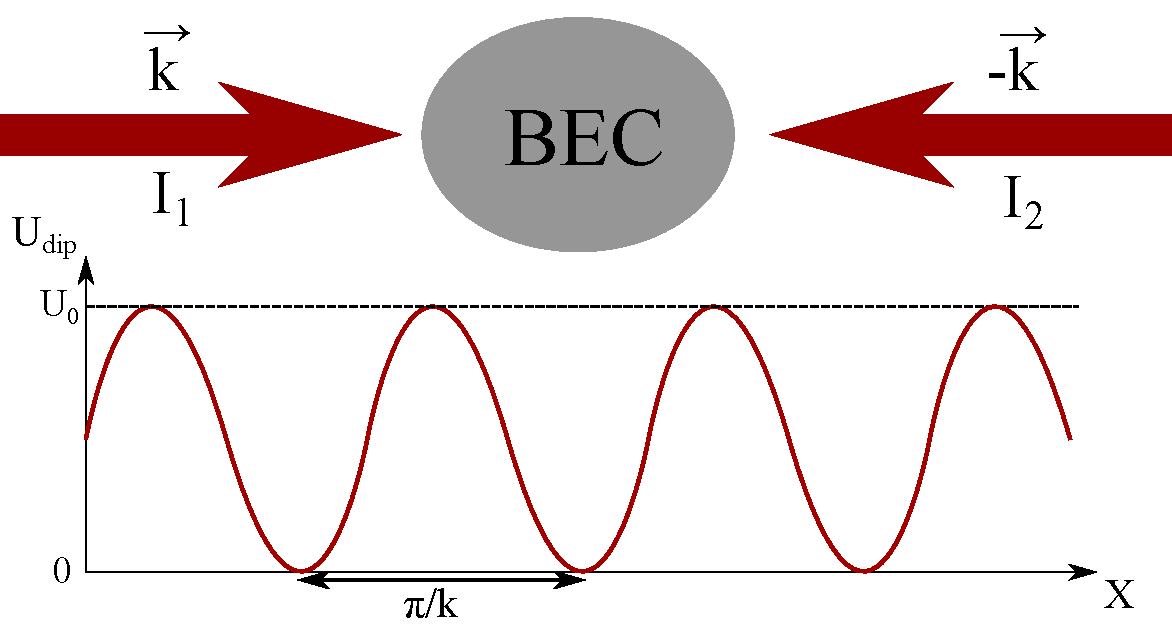
\includegraphics[width=1.\columnwidth]{lattice_beams.pdf}
	\caption[Scheme of an atomic \ac{bec} interacting with a one dimensional optical lattice]{Scheme of an atomic \ac{bec} interacting with a one dimensional optical lattice. For this case, it has been decided that the optical lattice is generated by two counter-propagating laser beams with wave number $k$, detuned a certain value $\delta$ from the erbium \SI{841}{\nano\meter} transition. Most of the lattice characteristics can be tuned by simply adjusting the beam intensities $I_1$ and $I_2$.}\label{fig:lattice_beams}
\end{figure}

\subsubsection{Moving optical lattice}

Once the lattice potential were obtained for two beams with the same frequency, there is a relevant case of study for which this appreciation is not valid. This is the situation in which there is a small detuning $\Delta$ between both beams. In this case, an additional temporal phase is added to one of the electric fields in Equation \eqref{eq:relation_electric_fields}. This means that the temporally independent expression for the lattice potential of Equation \eqref{eq:relation_lattice_potential}, becomes temporally dependent with the form
\begin{equation}\label{eq:relation_moving_lattice_potential}
	U_{\text{lat}}(\vec{r},t) = U_{0}(\vec{r}) \cdot \text{cos}^2\bigg(kx-\frac{\Delta}{2}t\bigg)
\end{equation} 

Where the intensities have also been assumed to be of the same order $I_{1}(\vec{r}) \sim I_{2}(\vec{r})$. This way, the lattice becomes a periodic potential, which moves along the beam propagation axis with time. Allowing for a different interaction process with the atomic ensemble, which will be described in the following section.


\section{Diffraction of an ultracold atomic ensemble}

When an atomic \ac{bec} interacts with an optical lattice, there are multiple processes that may be involved. Therefore, different regimes will appear, based on the lattice properties and interaction time with the atomic ensemble. Some of the main ones, which will be discussed here, are related with diffraction processes of the atomic ensemble. These two are commonly known as the Bragg and Raman-Nath regimes, which will be discussed in this section \cite{Mueller2008,Ovchinnikov1999}. To give an idea of how this diffraction effects act over an atomic ensemble, its experimental set-up must be considered analogous to the well-known process of light diffraction. Figure \ref{fig:diffraction} shows this analogy between both processes, generating different orders (0th, $\pm$1st ...) as a result. All these orders must fulfil a theoretical restriction known as the Bragg condition, which was initially theorized only for light diffraction by a crystal lattice \cite{Bragg1913}. However, this condition is also valid for atomic diffraction, with the detuning $\Delta$ between optical lattice beams, acting as the restricted parameter.


\begin{figure}[!htbp]\centering
	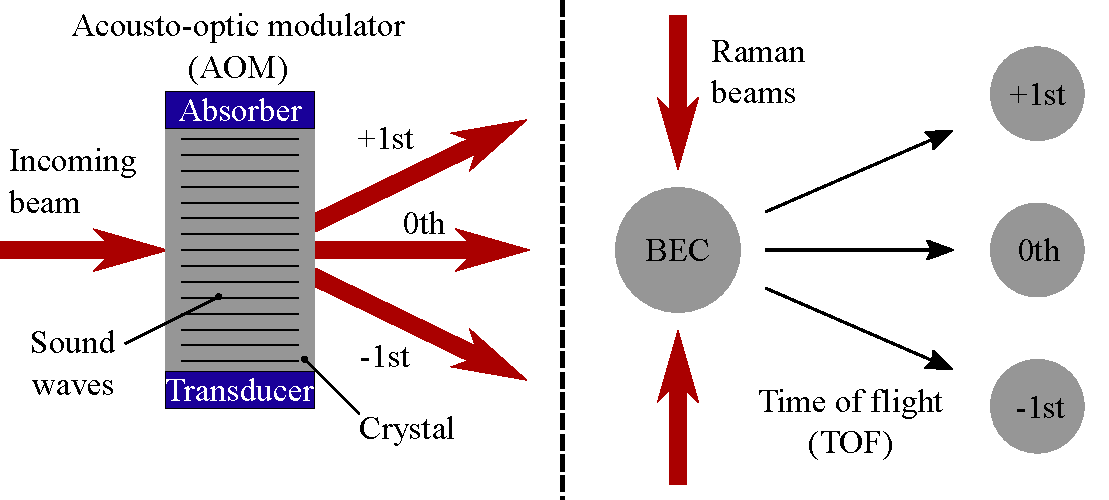
\includegraphics[width=1.\columnwidth]{diffraction.pdf}
	\caption[Analogy between the processes of light diffraction and atomic diffraction of an ultracold ensemble]{Analogy between the processes of light diffraction and atomic diffraction of an ultracold ensemble. The left side shows an light beam being diffracted through the use of an optical device commonly known as an \Acf{aom}. It consists on a solid-state crystal attached to a piezo-electric transducer, which generates sound waves responsible of diffracting the laser beam when it goes through the glass, acting as an optical medium. On the other hand, the right side shows the diffraction process of an atomic \ac{bec} produced by an optical lattice. The ensemble interacts during a certain interaction time $T_{\text{int}}$ with the optical lattice. After a waiting time known as \Acf{tof}, when the ensemble is just falling in vacuum due to gravity, the diffraction process takes place. For both cases, the result generates different orders (0th, $\pm$1st ...), which fulfil the so-called Bragg condition.}\label{fig:diffraction}
\end{figure}

\pagebreak

\subsection{Bragg condition}

To give an insight on the process leading to diffraction of an atomic ensemble into the $N$-th order, it is necessary to consider the physical scheme of a 2$N$-photon process. Therefore, the diffraction of an ultracold atomic \ac{bec} can be viewed as a stimulated Raman transition process \cite{Kozuma1999}. Meaning that one can think of the interaction between light and atoms, as photons from one beam being absorbed by the atomic ensemble while the other beam stimulates the emission of photons. This results in a momentum transfer into the ensemble, which is always ``kicked'' an invariant momentum quantity in every of this 2-photon interaction. However, in a 2$N$-photon process, every on this $N$-momentum transfers is produced in the optical lattice axis with a 50$\%$ chance of being in one direction or the other. This explains the appearance of multiple orders in the diffraction process, they are a result of the different 2$N$-photon interactions that the atoms inside an ensemble can produce. Moreover, it also explains why the separation between orders is the same, it is the displacement produced by the momentum transfer resulting from a 2-photon process after a \ac{tof}. This momentum transfer is commonly known as the 2-photon recoil $\vec{P}_\text{rec}$. To illustrate this, an atom must be considered with mass $M$ and initial momentum $\vec{P}_0 = \hbar \vec{k}_0$ along the lattice $x$-axis. The atom interacts with two photons, one coming from the left beam with momentum $\hbar \vec{k}_1$ and other from the right beam with $\hbar \vec{k}_2$. Thus, the total initial momentum of the system before interacting can be expressed as
\begin{equation}
	\vec{P}_\text{i} = \hbar \vec{k}_0 + \hbar (\vec{k}_1 + \vec{k}_2)
\end{equation}

And the total energy before interaction can also be obtained as
\begin{equation}\label{eq:bragg_energy_initial}
	E_\text{i} = \frac{\mathopen\big|\vec{P}_0\mathclose\big|^2}{2M} + \hbar (\omega_1 + \omega_2)
\end{equation}

After interacting, the atom absorbs one of the photons and is stimulated by the other. Resulting in the emission of two identical photons in one of the directions. Arbitrarily, the left photon will considered to be absorbed, hence the right one will be stimulated. The total momentum after interaction results
\begin{equation}
	\vec{P}_\text{f} = \hbar \vec{k}_0 + \hbar (\vec{k}_1 + \vec{k}_2) + 2\hbar\vec{k}_2
\end{equation}

The total energy can be obtained analogously like 
 \begin{equation}\label{eq:bragg_energy_final}
 	E_\text{f} = \frac{\mathopen\big|\vec{P}_0+\vec{P}_\text{rec}\mathclose\big|^2}{2M} + 2\hbar\omega_2
 \end{equation}
 
Where $\vec{P}_\text{rec} = \hbar (\vec{k}_1 + \vec{k}_2)$ represents the 2-photon recoil, the momentum transfer to the atom. It is usually reasonable to consider the case in which both beams forming the lattice have approximately the same wave number $\mathopen\big|\vec{k}_1\mathclose\big| \simeq \mathopen\big|\vec{k}_2\mathclose\big| \equiv k$. Even though, the beam frequencies differ a given value $\Delta$, this parameter is going to be small enough, allowing for the defined approximation. Due to this, an expression for the 2-photon recoil absolute value can be obtained as
\begin{equation}\label{eq:two_photon_recoil}
	\mathopen\big|\vec{P}_\text{rec}\mathclose\big| = 2 \hbar k \text{sin}\bigg(\frac{\theta}{2}\bigg)
\end{equation}

With $\theta$ the angle between wave vectors $\vec{k}_1$ and $\vec{k}_2$, and $k=\frac{2\pi}{\lambda}$ the wave number with wavelength $\lambda$.

By using the energy conservation principle with Equations \eqref{eq:bragg_energy_initial} and \eqref{eq:bragg_energy_final}, the resulting expression gives
\begin{equation}\label{eq:Bragg_condition_1}
	 \Delta_1 = \frac{1}{2M\hbar}\bigg[\mathopen\big|\vec{P}_{\text{rec}}\mathclose\big|^2 + 2\big(\vec{P}_0 \cdot \vec{P}_{\text{rec}}\big)\bigg]
\end{equation}

This gives the value for which the frequency difference between beams $\Delta = \omega_1-\omega_2$, fulfils the so-called Bragg condition in a 2-photon process. Therefore when $\Delta = \pm\Delta_1$, the $\pm1$st diffracted order becomes resonant, meaning that the physical system would tend to diffract more atoms into this order. Due to this, one can conclude that the Bragg condition in this experiment restricts $\Delta$ and therefore the moving lattice speed, which is governed by Equation \eqref{eq:relation_moving_lattice_potential}. The situation can be compared with the light diffraction process described in Figure \ref{fig:diffraction} for an \ac{aom}, with the incidence angle of the incoming beam playing the role of $\Delta$. When this angle fulfils the Bragg condition for the 1st order, it becomes resonant and most of the light will be diffracted through it. 

It can be proved that Equation \eqref{eq:Bragg_condition_1} generalized for a 2$N$-photon has the expression \cite{Kozuma1999}
\begin{equation}\label{eq:Bragg_condition_n}
	\Delta_n = \frac{1}{2M\hbar} \Bigg[n P_{\text{rec}}^2 + \frac{2\big(\vec{P}_0 \cdot \vec{P}_{\text{rec}}\big)}{n}\Bigg]
\end{equation}

Where $n=\pm1, \pm2, \text{...}$ for the different possible diffracted orders. It must be noted that the vectorial product $\vec{P}_0 \cdot \vec{P}_{\text{rec}}$ from Equation \eqref{eq:Bragg_condition_n} becomes zero in average for most of the cases. This is due to the fact that an atomic \ac{bec} can be considered static with respect to the optical lattice during the interaction time $T_{\text{int}}$. Thus, the resonance condition for the different orders can be obtained from Equations \eqref{eq:two_photon_recoil} and \eqref{eq:Bragg_condition_n} as
\begin{equation}
	\Delta_n = \frac{2n\hbar k^2}{M}
\end{equation}

For a lattice formed by two counter-propagating waves.

\subsection{Rabi oscillations}

As it has already been said, the diffraction of an atomic \ac{bec} with optical lattices can be considered as a 2$N$-photon process. This mean that the system behaviour relates 

\cite{Kozuma1999,Martin1988,Giltner1995}

\newpage

\section{Different regimes}

%besides the 2$n$-photon process can be 

%%% Local Variables: 
%%% mode: latex
%%% TeX-master: "Thesis"
%%% End: 
